%GiG
\documentclass{beamer} 
\usetheme{Copenhagen}
\setbeamertemplate{navigation symbols}{}
\setbeamertemplate{headline}{}
\DeclareMathOperator*{\argmax}{arg\,max}

\usepackage{hyperref}


\definecolor{azure}{rgb}{0.0, 0.5, 1.0}
%\newcommand{\tblue}[1]{\textcolor{blue}{#1}}
\newcommand{\tblue}[1]{{\Large {\textcolor{azure}{#1}}}}
\newcommand{\thblue}[1]{{\Huge {\textcolor{azure}{#1}}}}
\newcommand{\hred}[1]{{\textcolor{red}{#1}}}
\newcommand{\furl}[1]{{\footnote{\url{#1}}}}

\title[Saravanan Thirumuruganathan] 
{Lecture 7: Binary Heaps, Heapsort, Union-Find}

\author[CSE 5311] 
{Instructor: Saravanan Thirumuruganathan}

\date[] 

\begin{document}

\begin{frame}
  \titlepage
\end{frame}

%\begin{frame}{Outline}
%  \tableofcontents
%  % You might wish to add the option [pausesections]
%\end{frame}

\section{Outline}

\begin{frame}
\frametitle {Outline}
\begin{enumerate}
\item Data Structures to speed up algorithms 
\begin{itemize}
    \item Binary Heap
    \begin{itemize}
        \item Heapsort
    \end{itemize}
    \item Union Find
\end{itemize}
\end{enumerate}
\end{frame}

\begin{frame}{In-Class Quizzes}
\begin{itemize}
\item {\Large {\bf URL:}} {\LARGE \bf \url{http://m.socrative.com/}} 
\item {\Large {\bf Room Name:} {\LARGE \bf 4f2bb99e}}
\end{itemize}
\end{frame}

\section{General}

\begin{frame}{Data Structures}

\tblue{Key Things to Know for Data Structures}
\begin{itemize}
    \item Motivation
    \item Distinctive Property
    \item Major operations
    \item Key Helper Routines
    \item Representation
    \item Algorithms for major operations
    \item Applications
\end{itemize}
\end{frame}

\section{Binary Heap}

\begin{frame}{Data Structures for Algorithmic Speedup}
    \begin{itemize}
        \item BST and RBT are two examples of data structures to represent dynamic set
        \item Today's topic, Heap and Union-Find, can also be used to represent dynamic set
        \item However, these are used more often to speed up algorithms
    \end{itemize}
\end{frame}

\begin{frame}{}
    \begin{center}
        \thblue{Binary Heap}
    \end{center}
\end{frame}

\begin{frame}{Motivation}
    \begin{itemize}
        \item Heap Sort (CLRS is organized that way!)
        \item Priority Queue
        \item Most space efficient data structure
    \end{itemize}
\end{frame}

\begin{frame}{Priority Queue}
    \begin{itemize}
        \item ``Queue'' data structure has a FIFO property
        \item Some times it is useful to consider {\bf priority}
        \item Output element with highest priority first
    \end{itemize}
\end{frame}

\begin{frame}{Priority Queue - Major Operations}
    \begin{itemize}
        \item Insert
        \item FindMin (resp. FindMax)
        \item DeleteMin (resp. DeleteMax) 
        \item DecreaseKey (resp. IncreaseKey)
    \end{itemize}
\end{frame}

\begin{frame}{Priority Queue - Applications\footnote{{Kleinberg-Tardos Book and Wikipedia}}}
    \begin{itemize}
        \item Dijkstra's shortest path algorithm
        \item Prim's MST algorithm
        \item Heapsort
        \item Online median
        \item Huffman Encoding
        \item A* Search (or any Best first search)
        \item Discrete event simulation
        \item CPU Scheduling
        \item $\ldots$
        \item See Wikipedia entry for priority for details
    \end{itemize}
\end{frame}

\begin{frame}{Priority Queue - Candidate Implementations}
    \begin{itemize}
        \item Assume: for DeleteMin and DecreaseKey, pointer to element is given
        \item LinkedList
        \begin{itemize}
            \item Insert: \pause $O(1)$
            \item FindMin: \pause $O(n)$
            \item DeleteMin: \pause $O(1)$
            \item DecreaseKey: \pause $O(1)$
        \end{itemize}
        \item Binary Heap 
        \begin{itemize}
            \item Insert: $O(\lg n)$
            \item FindMin: $O(1)$
            \item DeleteMin: $O(\lg n)$
            \item DecreaseKey: $O(\lg n)$
        \end{itemize}
        \item Binomial Heaps, Fibonacci Heaps etc.
    \end{itemize}
\end{frame}

\begin{frame}{Binary Heaps}
    \begin{itemize}
        \item Perfect data structure for implementing Priority Queue
        \item MaxHeap and MinHeap
        \item We will focus on MaxHeaps in this lecture
    \end{itemize}
\end{frame}


\begin{frame}{Complete Tree\footnote{\url{http://www.cs.princeton.edu/courses/archive/spring13/cos423/lectures/BinomialHeaps.pdf}}}
    \begin{itemize}
        \item Perfectly balanced, except for bottom level
        \item Elements were inserted top-to-bottom and left-to-right
    \end{itemize}
    \begin{center}
        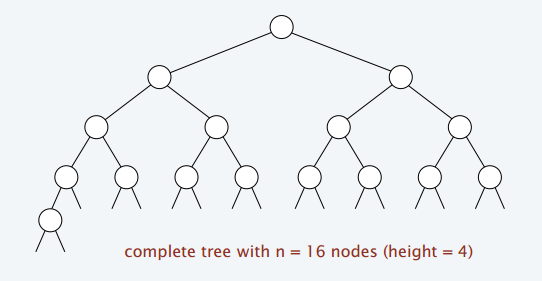
\includegraphics[scale=0.4]{completeTreeEg.png}
    \end{center}
\end{frame}

\begin{frame}{Heap Property}
    \begin{itemize}
        \item Heap is a binary tree ({\bf NOT BST})
        \item Heap:
        \begin{itemize}
            \item {\bf Completeness} Property: Heap has restricted structure. It must be a complete binary tree . 
            \item {\bf Ordering} Property: Relates parent value with that of its children
        \end{itemize}
        \item MaxHeap property: Value of parent must be greater than {\bf both} its children
        \item MinHeap property: Value of parent must be less than {\bf both} its children
        \item Heap with $n$ elements has height $O(\lg n)$
    \end{itemize}
\end{frame}

\begin{frame}{Max Heap Example\footnote{Wikipedia page for Heap}}
    \begin{center}
        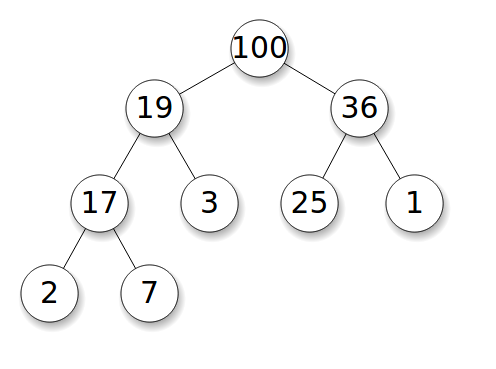
\includegraphics[scale=0.4]{maxHeapEg.png}
    \end{center}
\end{frame}


\begin{frame}{Heap Property\footnote{\url{http://courses.cs.washington.edu/courses/cse373/06sp/handouts/lecture10.pdf}}}
    \begin{center}
        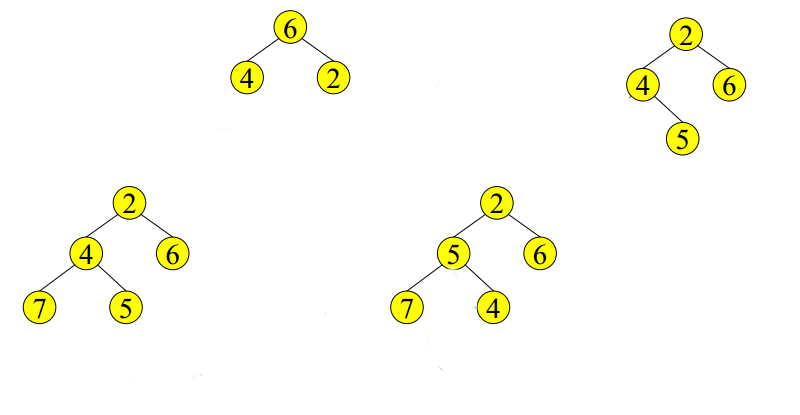
\includegraphics[scale=0.4]{heapOrNot.png}
    \end{center}
\end{frame}

\begin{frame}{Major Operations}
    \begin{itemize}
        \item Insert
        \item FindMax 
        \item DeleteMax (aka ExtractMax)
        \item IncreaseKey
    \end{itemize}
\end{frame}

\begin{frame}{Key Helper Routines}
    \begin{itemize}
        \item Max-Heapify (or Min-Heapify)
        \item Bubble-Up
        \item Bubble-Down
        \item Heapify
    \end{itemize}
\end{frame}

\begin{frame}{Representation: Arrays}
    \begin{itemize}
        \item Very efficient implementation using arrays
        \item Possible due to completeness property
        \item Parent($i$): return $\lfloor i/2 \rfloor$
        \item LeftChild($i$): return $2i$
        \item RightChild($i$): return $2i+1$
    \end{itemize}
\end{frame}

\begin{frame}{Representation: Arrays\footnote{CLRS Fig 6.1}}
    \begin{center}
        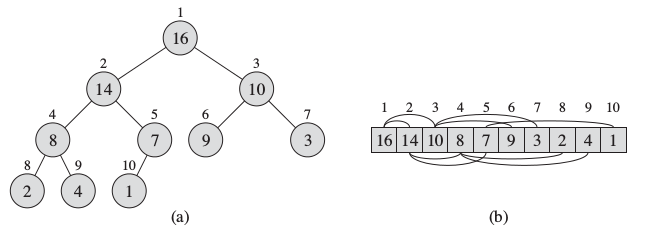
\includegraphics[scale=0.4]{maxHeapRepr.png}
    \end{center}
\end{frame}



\begin{frame}{Max-Heapify}
    \begin{itemize}
        \item Objective: Maintain heap property
        \item Invocation: Max-Heapify($A,i$)
        \item Assume: Left($i$) and Right($i$) are valid max-heaps
        \item $A[i]$ might violate max-heap property
        \item Bubble-Down the violation
        \item {\bf Analysis:} $O(\lg n)$
    \end{itemize}
\end{frame}


\begin{frame}{Max-Heapify: Example\footnote{CLRS Fig 6.2}}
    \begin{center}
        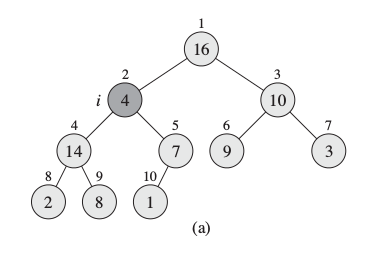
\includegraphics[scale=0.6]{maxHeapify1.png}
    \end{center}
\end{frame}


\begin{frame}{Max-Heapify: Example\footnote{CLRS Fig 6.2}}
    \begin{center}
        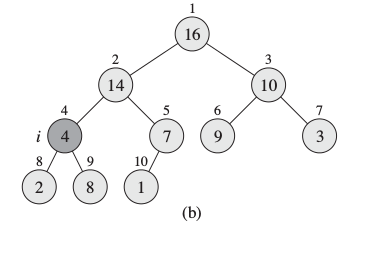
\includegraphics[scale=0.6]{maxHeapify2.png}
    \end{center}
\end{frame}


\begin{frame}{Max-Heapify: Example\footnote{CLRS Fig 6.2}}
    \begin{center}
        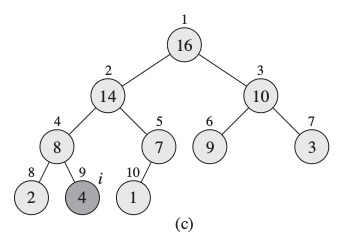
\includegraphics[scale=0.6]{maxHeapify3.png}
    \end{center}
\end{frame}

\begin{frame}{Heap : Insert}
    \begin{center}
        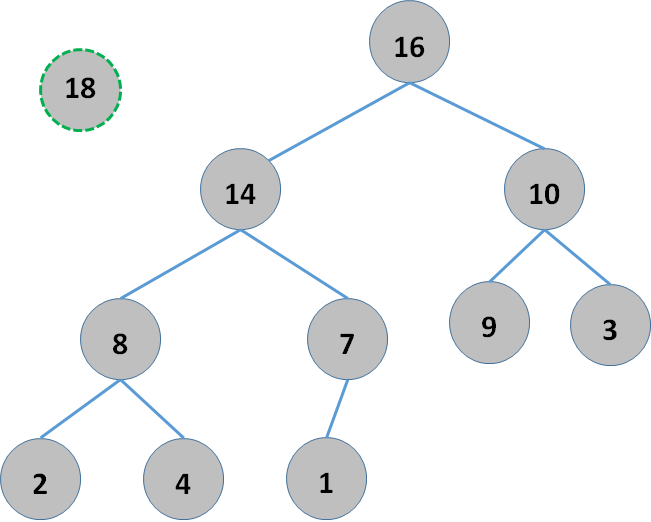
\includegraphics[scale=0.5]{heapInsert1.png}
    \end{center}
\end{frame}


\begin{frame}{Heap : Insert}
    \begin{center}
        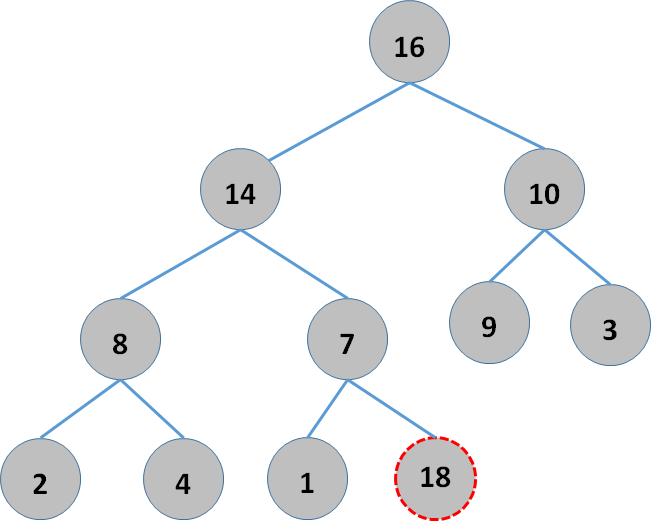
\includegraphics[scale=0.5]{heapInsert2.png}
    \end{center}
\end{frame}


\begin{frame}{Heap : Insert}
    \begin{center}
        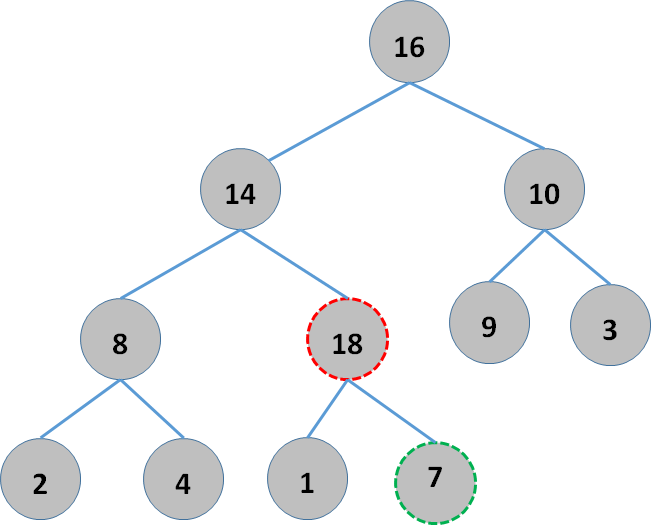
\includegraphics[scale=0.5]{heapInsert3.png}
    \end{center}
\end{frame}


\begin{frame}{Heap : Insert}
    \begin{center}
        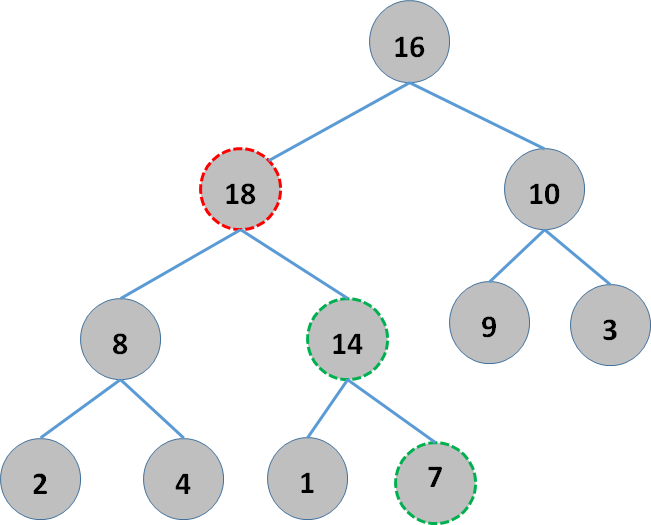
\includegraphics[scale=0.5]{heapInsert4.png}
    \end{center}
\end{frame}


\begin{frame}{Heap : Insert}
    \begin{center}
        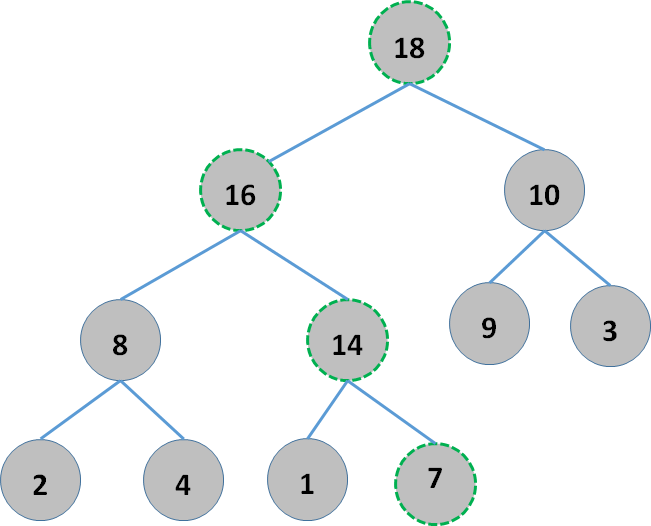
\includegraphics[scale=0.5]{heapInsert5.png}
    \end{center}
\end{frame}

\begin{frame}{Heap : Insert}
    \begin{itemize}
        \item Insert element at first available slot (no completeness property violation!)
        \item Fix heap property violations by bubbling up the vilolation till it is fixed
        \item Complexity: \pause $O(\lg n)$
    \end{itemize}
\end{frame}

\begin{frame}{Heap : FindMax}
    \begin{itemize}
        \item Look at the root element
        \item Time complexity: $O(1)$
    \end{itemize}
\end{frame}

\begin{frame}{Heap : DeleteMax}
    \begin{itemize}
        \item Delete the maximum element (root)
        \item Fix the heap
    \end{itemize}
\end{frame}

\begin{frame}{Heap : DeleteMax}
    \begin{center}
        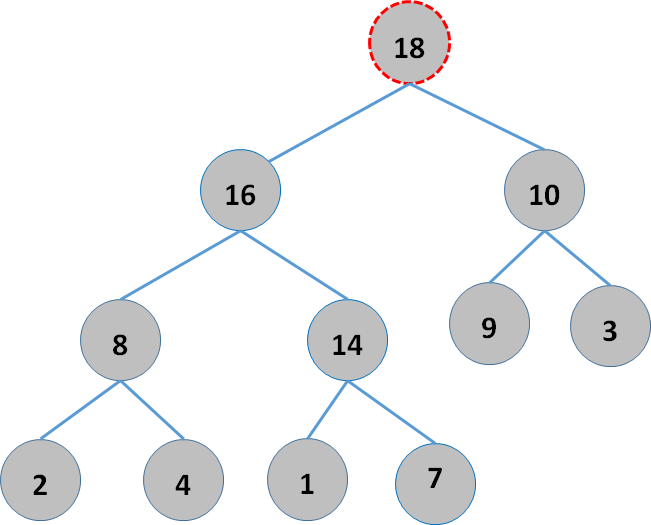
\includegraphics[scale=0.5]{heapDelete1.png}
    \end{center}
\end{frame}


\begin{frame}{Heap : DeleteMax}
    \begin{center}
        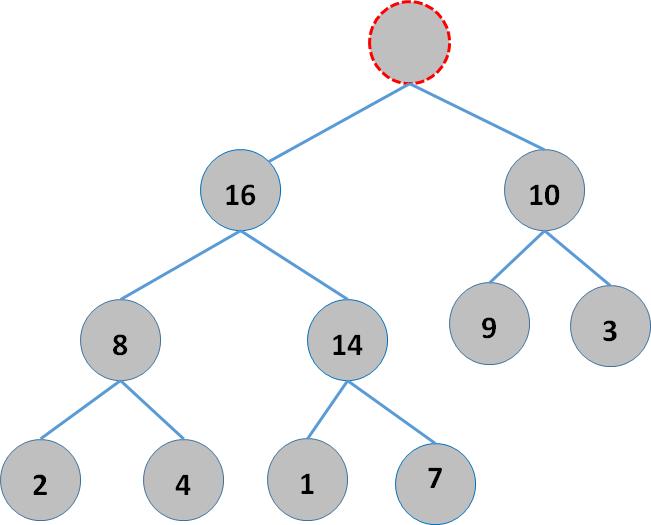
\includegraphics[scale=0.5]{heapDelete2.png}
    \end{center}
\end{frame}


\begin{frame}{Heap : DeleteMax}
    \begin{center}
        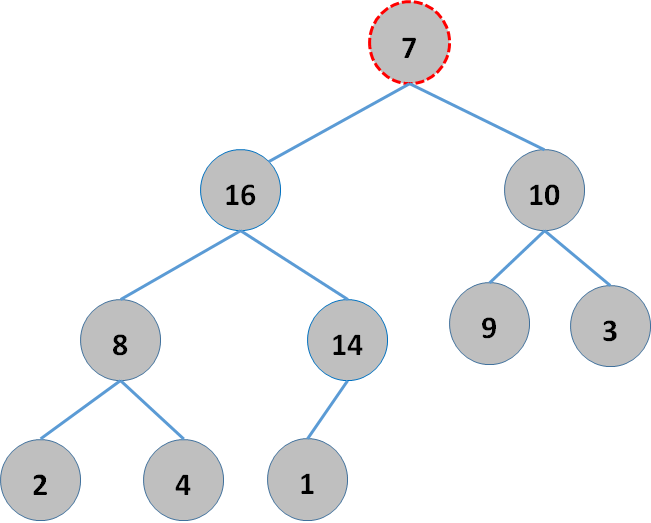
\includegraphics[scale=0.5]{heapDelete3.png}
    \end{center}
\end{frame}



\begin{frame}{Heap : DeleteMax}
    \begin{center}
        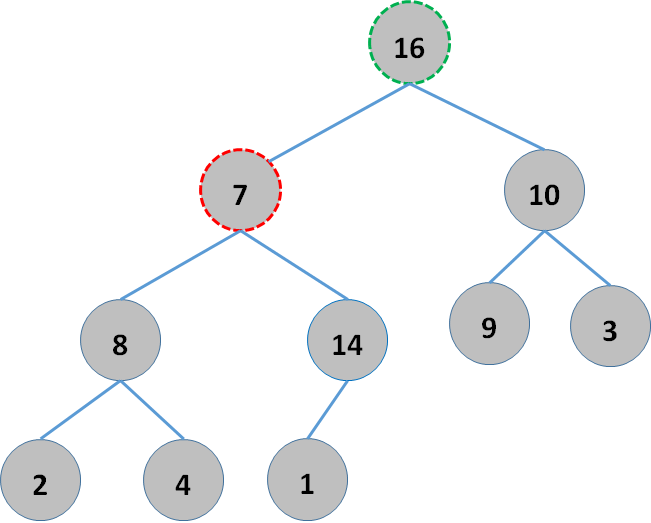
\includegraphics[scale=0.5]{heapDelete4.png}
    \end{center}
\end{frame}



\begin{frame}{Heap : DeleteMax}
    \begin{center}
        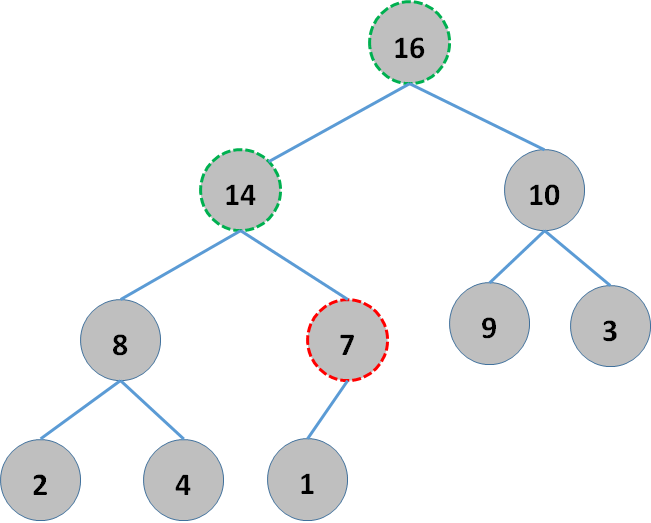
\includegraphics[scale=0.5]{heapDelete5.png}
    \end{center}
\end{frame}



\begin{frame}{Heap : DeleteMax}
    \begin{center}
        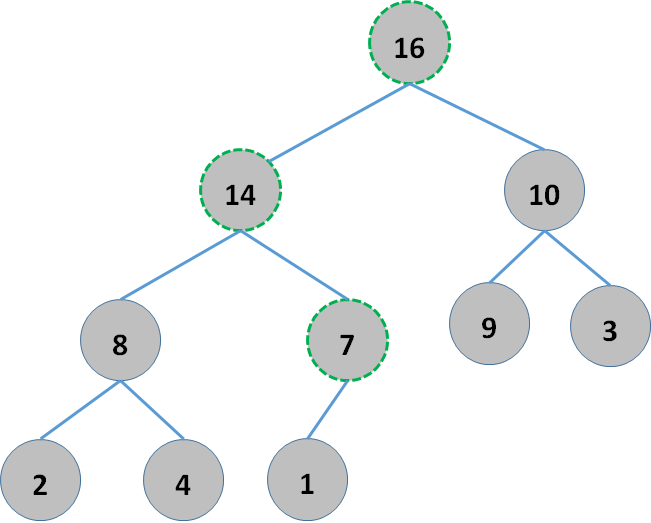
\includegraphics[scale=0.5]{heapDelete6.png}
    \end{center}
\end{frame}


\begin{frame}{Heap : DeleteMax}
    \begin{itemize}
        \item Remove root
        \item Replace root with last element (does not affect Completeness property)
        \item Fix heap violations by bubbling it down till it is fixed
        \item Complexity: \pause $O(\lg n)$
    \end{itemize}
\end{frame}


\begin{frame}{Heap : IncreaseKey}
    \begin{itemize}
        \item Given a node, increase its priority to a new, higher value
        \item Fix heap property violations 
    \end{itemize}
\end{frame}


\begin{frame}{Heap : IncreaseKey\footnote{CLRS Fig 6.5}}

\tblue{IncreaseKey:} Increase value of $4$ to $15$
    \begin{center}
        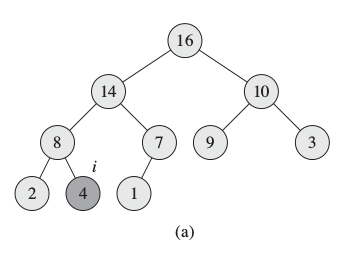
\includegraphics[scale=0.5]{heapIncreaseKey1.png}
    \end{center}
\end{frame}


\begin{frame}{Heap : IncreaseKey\footnote{CLRS Fig 6.5}}
    \begin{center}
        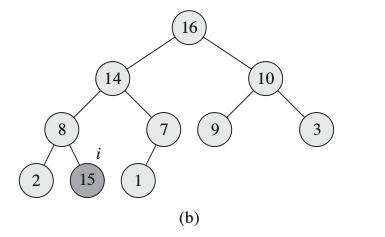
\includegraphics[scale=0.5]{heapIncreaseKey2.png}
    \end{center}
\end{frame}


\begin{frame}{Heap : IncreaseKey\footnote{CLRS Fig 6.5}}
    \begin{center}
        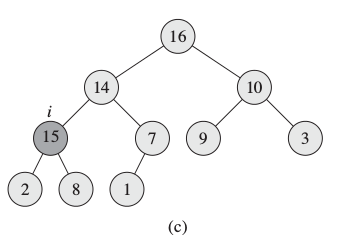
\includegraphics[scale=0.5]{heapIncreaseKey3.png}
    \end{center}
\end{frame}

\begin{frame}{Heap : IncreaseKey\footnote{CLRS Fig 6.5}}
    \begin{center}
        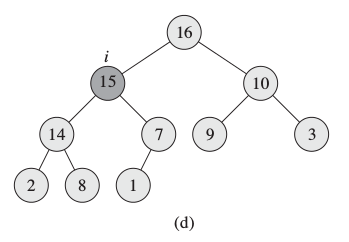
\includegraphics[scale=0.5]{heapIncreaseKey4.png}
    \end{center}
\end{frame}


\begin{frame}{Heap : IncreaseKey}
    \begin{itemize}
        \item Update element 
        \item Fix heap violations by bubbling it up till it is fixed
        \item Complexity: \pause $O(\lg n)$
    \end{itemize}
\end{frame}

\begin{frame}{Build-Max-Heap}
    \begin{itemize}
        \item Given an array $A$, convert it to a max-heap
        \item $A.length$: Length of the array
        \item $A.heapSize$: Elements from 1 $\ldots$ A.heapSize form a heap
        \item Build-Max-Heap($A$):
        \begin{itemize}
            \item A.heapSize = A.length
            \item for $i = \lfloor A.length / 2 \rfloor$ down to $1$ \\ \qquad Max-Heapify($A,i$)
        \end{itemize}
        \item {\bf Analysis:} $O(n)$ (See book for details)
    \end{itemize}
\end{frame}


\begin{frame}{Build-Max-Heap : Example \footnote{CLRS Fig 6.3}}
    \begin{center}
        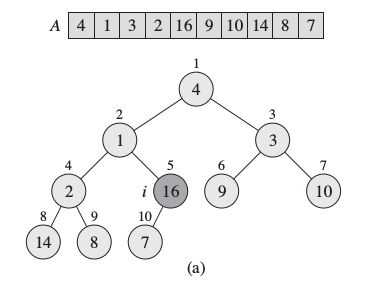
\includegraphics[scale=0.5]{buildMaxHeap1.png}
    \end{center}
\end{frame}


\begin{frame}{Build-Max-Heap : Example \footnote{CLRS Fig 6.3}}
    \begin{center}
        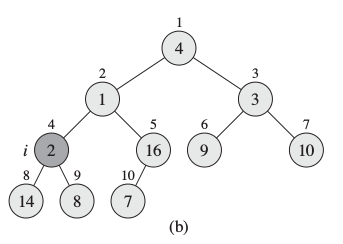
\includegraphics[scale=0.5]{buildMaxHeap2.png}
    \end{center}
\end{frame}


\begin{frame}{Build-Max-Heap : Example \footnote{CLRS Fig 6.3}}
    \begin{center}
        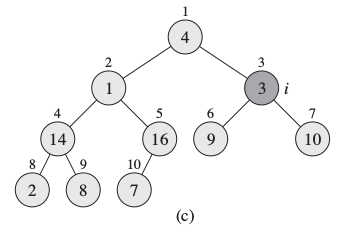
\includegraphics[scale=0.5]{buildMaxHeap3.png}
    \end{center}
\end{frame}


\begin{frame}{Build-Max-Heap : Example \footnote{CLRS Fig 6.3}}
    \begin{center}
        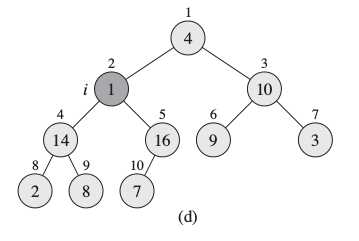
\includegraphics[scale=0.5]{buildMaxHeap4.png}
    \end{center}
\end{frame}


\begin{frame}{Build-Max-Heap : Example \footnote{CLRS Fig 6.3}}
    \begin{center}
        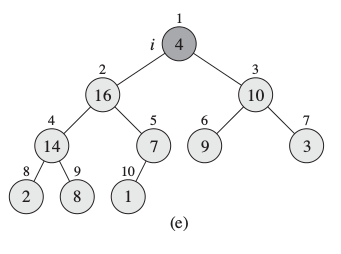
\includegraphics[scale=0.5]{buildMaxHeap5.png}
    \end{center}
\end{frame}


\begin{frame}{Build-Max-Heap : Example \footnote{CLRS Fig 6.3}}
    \begin{center}
        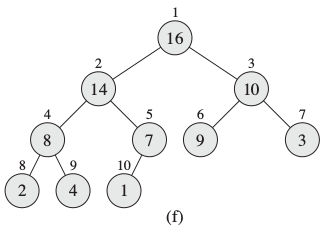
\includegraphics[scale=0.5]{buildMaxHeap6.png}
    \end{center}
\end{frame}


\section{Heapsort}
\begin{frame}[fragile]{HeapSort}
    \begin{verbatim}
    HeapSort(A):
        Build-Max-Heap(A)
        for i = A.length down to 2
            Exchange A[1] with A[i]
            A.heapSize = A.heapSize - 1
            Max-Heapify(A, 1)
    \end{verbatim}
\end{frame}


\begin{frame}{Heap Sort: Example\footnote{CLRS Fig 6.4}}
    \begin{center}
        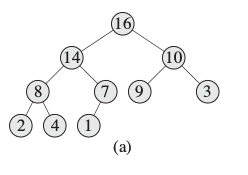
\includegraphics[scale=0.7]{heapSort1.png}
    \end{center}
\end{frame}


\begin{frame}{Heap Sort: Example\footnote{CLRS Fig 6.4}}
    \begin{center}
        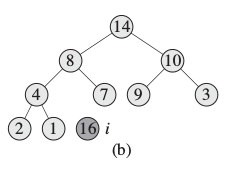
\includegraphics[scale=0.7]{heapSort2.png}
    \end{center}
\end{frame}


\begin{frame}{Heap Sort: Example\footnote{CLRS Fig 6.4}}
    \begin{center}
        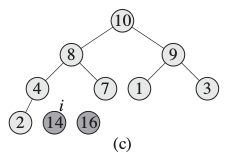
\includegraphics[scale=0.7]{heapSort3.png}
    \end{center}
\end{frame}


\begin{frame}{Heap Sort: Example\footnote{CLRS Fig 6.4}}
    \begin{center}
        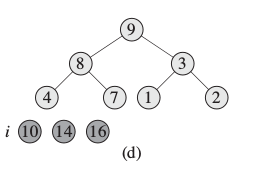
\includegraphics[scale=0.7]{heapSort4.png}
    \end{center}
\end{frame}


\begin{frame}{Heap Sort: Example\footnote{CLRS Fig 6.4}}
    \begin{center}
        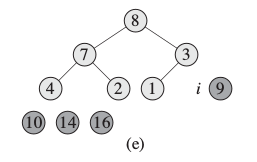
\includegraphics[scale=0.7]{heapSort5.png}
    \end{center}
\end{frame}


\begin{frame}{Heap Sort: Example\footnote{CLRS Fig 6.4}}
    \begin{center}
        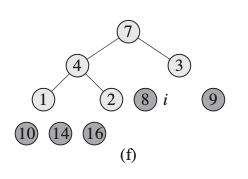
\includegraphics[scale=0.7]{heapSort6.png}
    \end{center}
\end{frame}


\begin{frame}{Heap Sort: Example\footnote{CLRS Fig 6.4}}
    \begin{center}
        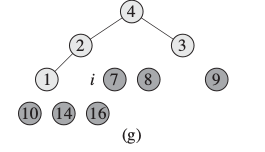
\includegraphics[scale=0.7]{heapSort7.png}
    \end{center}
\end{frame}


\begin{frame}{Heap Sort: Example\footnote{CLRS Fig 6.4}}
    \begin{center}
        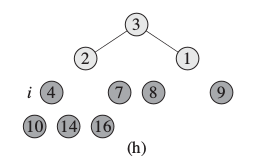
\includegraphics[scale=0.7]{heapSort8.png}
    \end{center}
\end{frame}


\begin{frame}{Heap Sort: Example\footnote{CLRS Fig 6.4}}
    \begin{center}
        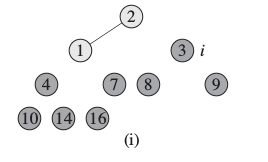
\includegraphics[scale=0.7]{heapSort9.png}
    \end{center}
\end{frame}


\begin{frame}{Heap Sort: Example\footnote{CLRS Fig 6.4}}
    \begin{center}
        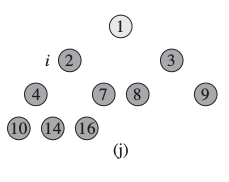
\includegraphics[scale=0.7]{heapSort10.png}
    \end{center}
\end{frame}


\begin{frame}{Heap Sort: Example\footnote{CLRS Fig 6.4}}
    \begin{center}
        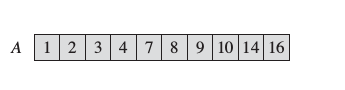
\includegraphics[scale=0.7]{heapSort11.png}
    \end{center}
\end{frame}


\begin{frame}{HeapSort: Analysis}
    \begin{itemize}
        \item Operations: 
        \begin{itemize}
            \item Build-Max-Heap: \pause $O(n)$
            \item $n$ Max-Heapify: \pause $n \times \lg n = O(n \lg n)$
            \item Complexity: $O(n) + O(n \lg n) = O(n \lg n)$
        \end{itemize}
    \end{itemize}
\end{frame}

\begin{frame}{HeapSort}
    \begin{itemize}
        \item Very efficient in practice - often competitive with QuickSort
        \item In-Place but not stable (why?)
        \item Requires constant extra space
        \item Best, average and worst case complexity is $O(n \lg n)$ (unlike Quicksort)
    \end{itemize}
\end{frame}

\section{Union-Find}

\begin{frame}{Data Structures for Disjoint Sets}
    \begin{center}
        \thblue{Data Structures for Disjoint Sets}
    \end{center}
\end{frame}

\begin{frame}{Disjoint Sets ADT}
    \begin{itemize}
        \item Objective: Represent and manipulate disjoint sets (sets that do not overlap)
        \item Required Operations
        \begin{itemize}
            \item MakeSet($x$): Create a new set $\{x\}$ with single element $x$
            \item Find($x$): Find the set containing $x$
            \item Union($x,y$): Merge sets containing $x$ and $y$
        \end{itemize}
    \end{itemize}
\end{frame}

\begin{frame}{Disjoint Sets: Example\footnote{\url{https://www.cs.princeton.edu/~rs/AlgsDS07/01UnionFind.pdf}}}
    \begin{center}
        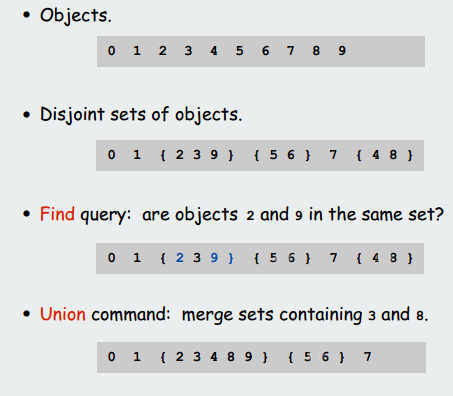
\includegraphics[scale=0.5]{disjointSetEg.png}
    \end{center}
\end{frame}

\begin{frame}{Disjoint Sets: Applications\footnote{\url{http://courses.cs.washington.edu/courses/cse326/08sp/lectures/18-disjoint-union-find.pdf}}}
    \begin{itemize}
        \item Network connectivity: are two computers connected? 
        \item Compilers: are two variables aliases?
        \item Image segmentation: are both pixels in same segment?
        \item Chip design: are two transistors connected to each other?
        \item Maze design
        \item Speeding up Kruskal's MST algorithm
        \item Many many more
    \end{itemize}
\end{frame}

\begin{frame}{Disjoint Sets: Naming}
    \begin{itemize}
        \item Represent each disjoint set by a unique name
        \item For convenience, the name is one of its elements
        \item This element is called the {\bf leader} of the set
        \item Find($x$) returns the leader of set containing $x$
        \item Typically, Union takes leaders as input. For eg, Union($a,b$). If not easily fixable by Union(Find($a$), Find($b$)) 
    \end{itemize}
\end{frame}

\begin{frame}{Data Structures for Disjoint Sets}

    {\bf Objective:} 
    \begin{itemize}
        \item Design an efficient data structure to represent DS ADT 
        \item Assume that there are $N$ elements - represented by $1, \ldots, N$
        \item $M$ operations (any mixture of union and find)
    \end{itemize}
    {\bf Candidate Representations:}
    \begin{itemize}
        \item Array based
        \item Linked List based
        \item Tree based
    \end{itemize}
\end{frame}

\begin{frame}{Disjoint Sets Implementation: Arrays}

        {\bf Idea:} 
        \begin{itemize}
            \item Maintain an array $A$ with $N$ elements
            \item $A[i]$ stores the leader for set containing element $i$
        \end{itemize}

        {\bf Find:} Find($3$)=$4$, Find($6$)=$8$ 
        \begin{center}
            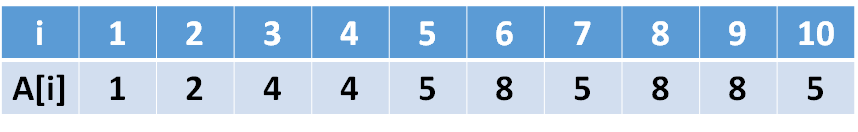
\includegraphics[scale=0.4]{unionFindArray1.png}
        \end{center}
        {\bf Union:} Union($4,8$)
        \begin{center}
            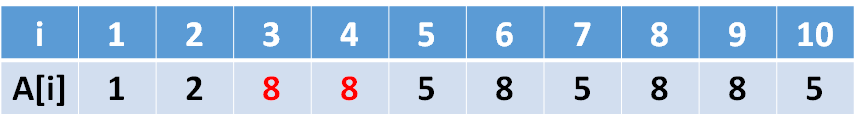
\includegraphics[scale=0.4]{unionFindArray2.png}
        \end{center}
\end{frame}

\begin{frame}{Disjoint Sets Implementation: Arrays}

    {\bf Analysis:}
    \begin{itemize}
        \item Find: \pause $O(1)$
        \item Union: \pause $O(N)$
        \item Complexity for $M$ operations: $O(MN)$
    \end{itemize}
\end{frame}

\begin{frame}{Disjoint Sets Implementation: Linked List\footnote{CLRS Fig 21.2}}

        {\bf Idea:} 
        \begin{itemize}
            \item Represent each set as a linked list
            \item Set first element of each linked list as the leader
        \end{itemize}

        \begin{center}
            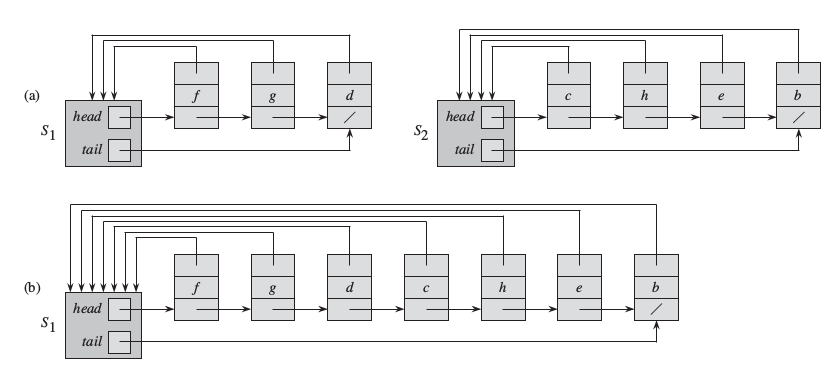
\includegraphics[scale=0.4]{unionFindLinkedList.png}
        \end{center}

\end{frame}

\begin{frame}{Disjoint Sets Implementation: Linked List}

    {\bf Analysis:}
    \begin{itemize}
        \item Find: \pause $O(1)$
        \item Union: \pause $O(N)$
        \item Complexity for $M$ operations: $O(MN)$
    \end{itemize}
\end{frame}

\begin{frame}{Disjoint Sets Implementation: Tree}
    \begin{itemize}
        \item Also called as Union-Find data structure
        \item Idea: Represent each set as a tree
        \item Store all sets as a forest (collection of disconnected trees)
        \item Allow each node to have arbitrary number of children
        \item Root of each tree is the leader
    \end{itemize}
\end{frame}

\begin{frame}{Union-Find: Up-Tree Representation\footnote{\url{http://courses.cs.washington.edu/courses/cse326/08sp/lectures/19-disjoint-union-find-part-2.pdf}}}
    \begin{center}
        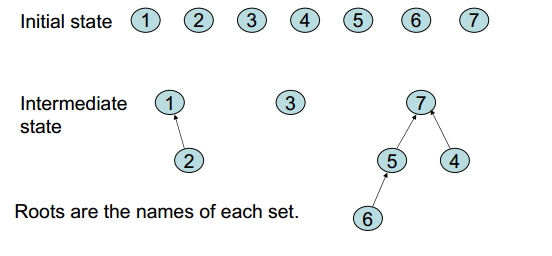
\includegraphics[scale=0.5]{unionFindTreeRep.png} 
    \end{center}
\end{frame}


\begin{frame}{Union-Find: Up-Tree Representation \footnote{\url{http://courses.cs.washington.edu/courses/cse326/08sp/lectures/19-disjoint-union-find-part-2.pdf}} }
    \begin{center}
        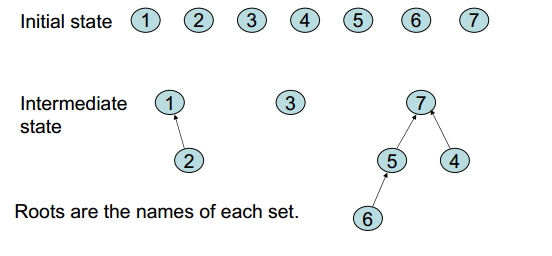
\includegraphics[scale=0.5]{unionFindTreeRep.png} 
    \end{center}
\end{frame}


\begin{frame}{Union-Find: Find Operation \footnote{\url{http://courses.cs.washington.edu/courses/cse326/08sp/lectures/19-disjoint-union-find-part-2.pdf}} } 
    \begin{center}
        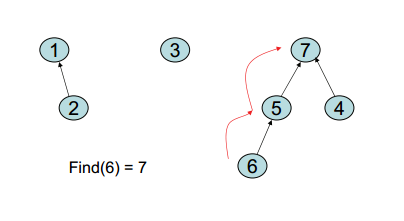
\includegraphics[scale=0.5]{unionFindTreeRepFind.png} 
    \end{center}
\end{frame}


\begin{frame}{Union-Find: Union Operation \footnote{\url{http://courses.cs.washington.edu/courses/cse326/08sp/lectures/19-disjoint-union-find-part-2.pdf}} }
    \begin{center}
        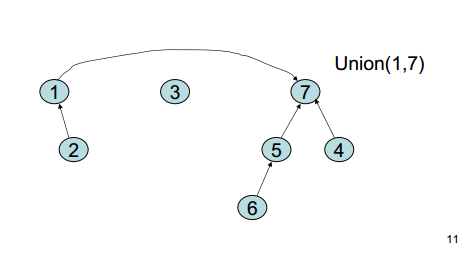
\includegraphics[scale=0.5]{unionFindTreeRepUnion.png} 
    \end{center}
\end{frame}


\begin{frame}{Union-Find: Up-Tree Implementation \footnote{\url{http://courses.cs.washington.edu/courses/cse326/08sp/lectures/19-disjoint-union-find-part-2.pdf}} }
    \begin{center}
        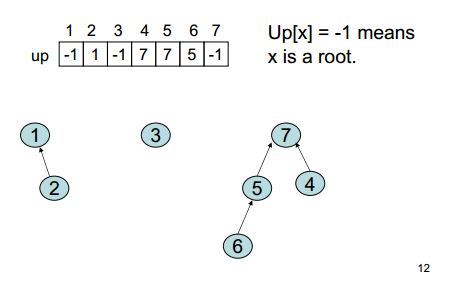
\includegraphics[scale=0.5]{unionFindTreeRepImplem.png} 
    \end{center}
\end{frame}


\begin{frame}{Union-Find: Worst Case\footnote{\url{http://courses.cs.washington.edu/courses/cse326/08sp/lectures/19-disjoint-union-find-part-2.pdf}} }
    \begin{center}
        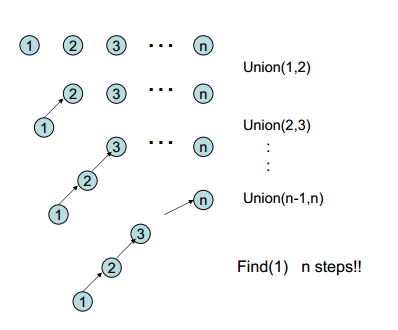
\includegraphics[scale=0.5]{unionFindWorstCase.png} 
    \end{center}
\end{frame}


\begin{frame}{Union-Find: Candidate Improvements}
    \begin{itemize}
        \item \pause Improve Union
        \begin{itemize}
            \item Union by Size
            \item Union by Rank (depth)
        \end{itemize}
        \item Improve Find
    \end{itemize}
\end{frame}


\begin{frame}{Union-Find: Improved Union\footnote{\url{http://courses.cs.washington.edu/courses/cse326/08sp/lectures/19-disjoint-union-find-part-2.pdf}}}

\tblue{Union by Size (Weighted Union):} Always point smaller tree to root of larger tree. Break ties arbitrarily.
    \begin{center}
        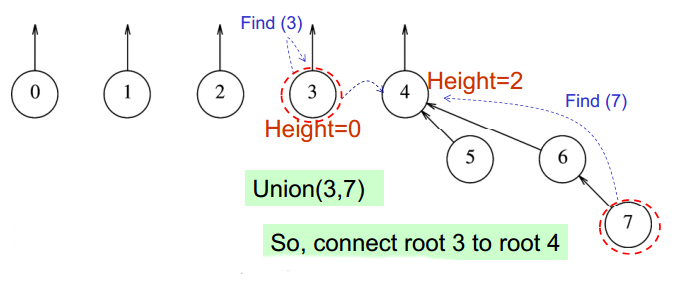
\includegraphics[scale=0.5]{unionByRank.png} 
    \end{center}
\end{frame}

\begin{frame}{Union-Find: Improved Union}

\tblue{Union by Rank:} Always point tree with smaller rank (depth) to root of larger tree. Break ties arbitrarily.
    \begin{center}
        \includegraphics[scale=0.5]{unionByRank.png} 
    \end{center}
\end{frame}

\begin{frame}{Union by Size: Best Case\footnote{\url{http://courses.cs.washington.edu/courses/cse326/08sp/lectures/19-disjoint-union-find-part-2.pdf}}}

    \begin{center}
        \includegraphics[scale=0.5]{unionByRankBestCase.png} 
    \end{center}

    {\bf Complexity:} \pause Union and Find take $O(1)$ time
\end{frame}

\begin{frame}{Union by Size: Worst Case\footnote{\url{http://courses.cs.washington.edu/courses/cse326/08sp/lectures/19-disjoint-union-find-part-2.pdf}}}
    \begin{center}
        \includegraphics[scale=0.5]{unionByRankWorstCase.png} 
    \end{center}
    {\bf Complexity:} \pause Union takes $O(1)$ and Find take $O(\lg n)$ time
\end{frame}


\begin{frame}{Union-Find: Improved Find\footnote{\url{http://courses.cs.washington.edu/courses/cse326/08sp/lectures/19-disjoint-union-find-part-2.pdf}}}

    \begin{center}
        \includegraphics[scale=0.5]{pathCompression1.png} 
    \end{center}
\end{frame}


\begin{frame}{Union-Find: Improved Find\footnote{\url{http://courses.cs.washington.edu/courses/cse326/08sp/lectures/19-disjoint-union-find-part-2.pdf}}}

    \tblue{Path Compression:} When doing find, point all nodes on search path to root.
    \begin{center}
        \includegraphics[scale=0.5]{pathCompression2.png} 
    \end{center}
\end{frame}

\begin{frame}{Union-Find: Improved Find\footnote{CLRS Fig 21.5}}
    \begin{center}
        \includegraphics[scale=0.3]{pathCompression4.png} 
    \end{center}
\end{frame}

\begin{frame}{Union-Find}
    \begin{itemize}
        \item Amortized analysis
        \item Similarity with Red-Black trees
        \item Worst Case Analysis of Union-by Size + Path Compression
        \begin{itemize}
            \item Single Union-by-Size:
            \item Single Find with Path Compression: 
            \item Amortized Complexity for $M \geq N$ operations: $O(m \log^{*} n)$
        \end{itemize}
    \end{itemize}
\end{frame}

\begin{frame}{$Log^{*}$ Function\footnote{\url{http://courses.cs.washington.edu/courses/cse326/08sp/lectures/19-disjoint-union-find-part-2.pdf}}}
    \begin{itemize}
        \item $\log^{*} 2 = 1$
        \item $\log^{*} 4 = \log^{*} 2^2 = 2$
        \item $\log^{*} 16 = \pause \log^{*} 2^{2^{2}} = 3$ (i.e. $\log \log \log 16 = 1$)
        \item $\log^{*} 65536 = \pause \log^{*} 2^{2^{2^{2}}} = 4$ (i.e. $\log \log \log \log 65536 = 1$)
        \item $\log^{*} 2^{65536} = \pause \ldots = 5$ (i.e. $\log \log \log \log \log 2^65536 = 1$)
        \item In summary for all reasonable $n$ , $\log^{*} n \leq 5 $
    \end{itemize}
\end{frame}


\begin{frame}{Tighter Bound}
    \begin{itemize}
        \item Tarjan's tighter bound when $M \geq N$, $\Theta( M \alpha(M, N))$
        \item $\alpha(a,b)$ is the inverse Ackerman function
        \item It grows even slower than $\log^{*} n$!
    \end{itemize}
\end{frame}

\section{Summary}

\begin{frame}{Summary}

\tblue{Major Concepts:}
\begin{itemize}
\item Binary Heap
\item Heapsort
\item Disjoint set data structures
\item Union-Find
\end{itemize}
\end{frame}


\end{document}

